\documentclass[twoside]{book}

% Packages required by doxygen
\usepackage{fixltx2e}
\usepackage{calc}
\usepackage{doxygen}
\usepackage[export]{adjustbox} % also loads graphicx
\usepackage{graphicx}
\usepackage[utf8]{inputenc}
\usepackage{makeidx}
\usepackage{multicol}
\usepackage{multirow}
\PassOptionsToPackage{warn}{textcomp}
\usepackage{textcomp}
\usepackage[nointegrals]{wasysym}
\usepackage[table]{xcolor}

% Font selection
\usepackage[T1]{fontenc}
\usepackage[scaled=.90]{helvet}
\usepackage{courier}
\usepackage{amssymb}
\usepackage{sectsty}
\renewcommand{\familydefault}{\sfdefault}
\allsectionsfont{%
  \fontseries{bc}\selectfont%
  \color{darkgray}%
}
\renewcommand{\DoxyLabelFont}{%
  \fontseries{bc}\selectfont%
  \color{darkgray}%
}
\newcommand{\+}{\discretionary{\mbox{\scriptsize$\hookleftarrow$}}{}{}}

% Page & text layout
\usepackage{geometry}
\geometry{%
  a4paper,%
  top=2.5cm,%
  bottom=2.5cm,%
  left=2.5cm,%
  right=2.5cm%
}
\tolerance=750
\hfuzz=15pt
\hbadness=750
\setlength{\emergencystretch}{15pt}
\setlength{\parindent}{0cm}
\setlength{\parskip}{3ex plus 2ex minus 2ex}
\makeatletter
\renewcommand{\paragraph}{%
  \@startsection{paragraph}{4}{0ex}{-1.0ex}{1.0ex}{%
    \normalfont\normalsize\bfseries\SS@parafont%
  }%
}
\renewcommand{\subparagraph}{%
  \@startsection{subparagraph}{5}{0ex}{-1.0ex}{1.0ex}{%
    \normalfont\normalsize\bfseries\SS@subparafont%
  }%
}
\makeatother

% Headers & footers
\usepackage{fancyhdr}
\pagestyle{fancyplain}
\fancyhead[LE]{\fancyplain{}{\bfseries\thepage}}
\fancyhead[CE]{\fancyplain{}{}}
\fancyhead[RE]{\fancyplain{}{\bfseries\leftmark}}
\fancyhead[LO]{\fancyplain{}{\bfseries\rightmark}}
\fancyhead[CO]{\fancyplain{}{}}
\fancyhead[RO]{\fancyplain{}{\bfseries\thepage}}
\fancyfoot[LE]{\fancyplain{}{}}
\fancyfoot[CE]{\fancyplain{}{}}
\fancyfoot[RE]{\fancyplain{}{\bfseries\scriptsize Generated by Doxygen }}
\fancyfoot[LO]{\fancyplain{}{\bfseries\scriptsize Generated by Doxygen }}
\fancyfoot[CO]{\fancyplain{}{}}
\fancyfoot[RO]{\fancyplain{}{}}
\renewcommand{\footrulewidth}{0.4pt}
\renewcommand{\chaptermark}[1]{%
  \markboth{#1}{}%
}
\renewcommand{\sectionmark}[1]{%
  \markright{\thesection\ #1}%
}

% Indices & bibliography
\usepackage{natbib}
\usepackage[titles]{tocloft}
\setcounter{tocdepth}{3}
\setcounter{secnumdepth}{5}
\makeindex

% Hyperlinks (required, but should be loaded last)
\usepackage{ifpdf}
\ifpdf
  \usepackage[pdftex,pagebackref=true]{hyperref}
\else
  \usepackage[ps2pdf,pagebackref=true]{hyperref}
\fi
\hypersetup{%
  colorlinks=true,%
  linkcolor=blue,%
  citecolor=blue,%
  unicode%
}

% Custom commands
\newcommand{\clearemptydoublepage}{%
  \newpage{\pagestyle{empty}\cleardoublepage}%
}

\usepackage{caption}
\captionsetup{labelsep=space,justification=centering,font={bf},singlelinecheck=off,skip=4pt,position=top}

%===== C O N T E N T S =====

\begin{document}

% Titlepage & ToC
\hypersetup{pageanchor=false,
             bookmarksnumbered=true,
             pdfencoding=unicode
            }
\pagenumbering{alph}
\begin{titlepage}
\vspace*{7cm}
\begin{center}%
{\Large Assignment1\+\_\+\+Exp\+\_\+\+Ro\+\_\+\+Lab }\\
\vspace*{1cm}
{\large Generated by Doxygen 1.8.13}\\
\end{center}
\end{titlepage}
\clearemptydoublepage
\pagenumbering{roman}
\tableofcontents
\clearemptydoublepage
\pagenumbering{arabic}
\hypersetup{pageanchor=true}

%--- Begin generated contents ---
\chapter{Assignment 1 -\/ Experimental Robotics Laboratory}
\label{md_README}
\Hypertarget{md_README}
\section*{Behavioral Architecture}

Assuming a Robot, simulating a pet, that interacts with a human and moves in a discrete 2D environment. The robot may have three behaviors \+: normal (in which it moves randomly), sleep (in which it gets the home position, sleeps for a time and returns in normal behavior) and play (in which it goes in person location, waits for a poiting gesture, goes in the pointed location, comes back to the person and waits for the next pointing gestures. After some time it returns to the normal behavior). The human can interact by pointing gestures and speech.

\subsection*{R\+OS Architecture}

The system is composed by 3 nodes\+:\char`\"{}\+Commander\char`\"{} node, \char`\"{}state\+\_\+machine\char`\"{} node and \char`\"{}\+Display\char`\"{} node, and a Launch file. The rqt\+\_\+graph is showed.

 

\subsubsection*{Commander node}

The node simulates user action. Firstly it chooses randomly what the robot must perform\+: sleep or play. The command (std\+\_\+msgs/\+String) is published on a Topic (\char`\"{}/\+Command\char`\"{}). In case the play behavior is selected, the node generates randomly the location of the user and the Pointing Gesture. These poses (geometry\+\_\+msgs/\+Point) are published on two topics (\char`\"{}/\+Person\+Position\char`\"{} and \char`\"{}/\+Pointing\+Gesture\char`\"{}).

\subsubsection*{State machine node}

The node implements a state machine in which the three possible behaviors are defined.

 

The state machine starts with a Normal behavior state, and it can transit to sleep state or to play state, or it can keep a normal state. The command to switch to another state is received by \char`\"{}\+Commander\char`\"{} node by the topic \char`\"{}/\+Command\char`\"{}. When it is in a Play state or in a Sleep state, it can just go back in the normal state. The R\+OS message geometry\+\_\+msgs/\+Point is used to rapresent the 2D robot\textquotesingle{}s position (leaving z component always equal to 0). The target position belongs exclusively to the map (11x11 grid). In the normal state, they are generated by \char`\"{}\+Generate\+Random\+Position\char`\"{} function; in the play state, the person position and pointing gesture are received by \char`\"{}\+Commander\char`\"{} node through two topics; while in the sleep state the home position is defined (1,1). For each state, the target positions are sent to the \char`\"{}display\char`\"{} node, publishing them on \char`\"{}\+New\+Target\+Position\char`\"{} topic. When this happens, the system waits for a default time (4 seconds) until the robot reaches the desired pose. This means that further targets has not been accepted while the robot is moving.

\subsubsection*{Display node}

The node is a simple simulator; it subscribes to a \char`\"{}new\+Target\+Position\char`\"{} topic and wait for a message. When the target is received, it prints on terminal what the robot is doing and the behavior state.

\subsection*{Installation}

The first thing to do, after having cloned the repository in the Ros workspace, is to build the package, using the following commands in the shell\+: \begin{DoxyVerb}```
cd "yourWorkspace"_ws
catkin_make

```
\end{DoxyVerb}
 To run the system\+: \begin{DoxyVerb}```
roslaunch assignment1_ExRoLab ass1.launch

```
\end{DoxyVerb}
 In another terminal run\+: \begin{DoxyVerb}```
rosrun assignment1_ExRoLab Commander.py 

```
\end{DoxyVerb}


To visualize the smach viewer\+: \begin{DoxyVerb}```
rosrun smach_viewer smach_viewer.py

```
\end{DoxyVerb}


\subsection*{Working Hypothesis}

The assumptions are\+: 1) When it starts, the normal state preempts other states. 2) From the normal behavior, the robot can play or sleep or stay in normal state yet. 3) The command to go to sleep or play is received by the Commander node. 4) From the play state, as well as from the sleep state, the robot can only go to the normal state. 5) The random position in the normal state is defined by \char`\"{}\+Generate\+Random\+Position\char`\"{} function. 6) The home position is fixed (1,1,0). 7) The person location and the pointing gesture are received by the Commander node. 8) During the execution of one state, after giving a target, the robot waits for a while (predefined time).

\subsection*{System\textquotesingle{}s features}

The sys can show on the terminal what the robot is doing and the what the behavior\textquotesingle{}s state is executing.

\subsection*{System\textquotesingle{}s Limitations}

The user actions is randomly defined by the system, and there exists neither a real relationship with the user nor a real pointing gesture. The robot has not a velocity to get him desired target position, and there is not a real simulator to view if the target is achieved.

\subsection*{Possible technical Improvements}

A possible technical improvements may be\+: 1) create a real interaction with the user; 2) Implement a real velocity to change the odometry of the robot; 4) Implement a simulator (like Gazebo, Stage, Turtlesim,...).

\subsection*{Author}

Sara Romano -\/ \href{mailto:sara.romano.15@gmail.com}{\tt sara.\+romano.\+15@gmail.\+com} 
\chapter{Hierarchical Index}
\section{Class Hierarchy}
This inheritance list is sorted roughly, but not completely, alphabetically\+:\begin{DoxyCompactList}
\item State\begin{DoxyCompactList}
\item \contentsline{section}{state\+\_\+machine.\+Normal}{\pageref{classstate__machine_1_1Normal}}{}
\item \contentsline{section}{state\+\_\+machine.\+Play}{\pageref{classstate__machine_1_1Play}}{}
\item \contentsline{section}{state\+\_\+machine.\+Sleep}{\pageref{classstate__machine_1_1Sleep}}{}
\end{DoxyCompactList}
\end{DoxyCompactList}

\chapter{Class Index}
\section{Class List}
Here are the classes, structs, unions and interfaces with brief descriptions\+:\begin{DoxyCompactList}
\item\contentsline{section}{\hyperlink{classstate__machine_1_1Normal}{state\+\_\+machine.\+Normal} \\*\hyperlink{classstate__machine_1_1Normal}{Normal} state definition }{\pageref{classstate__machine_1_1Normal}}{}
\item\contentsline{section}{\hyperlink{classstate__machine_1_1Play}{state\+\_\+machine.\+Play} \\*\hyperlink{classstate__machine_1_1Play}{Play} state definition }{\pageref{classstate__machine_1_1Play}}{}
\item\contentsline{section}{\hyperlink{classstate__machine_1_1Sleep}{state\+\_\+machine.\+Sleep} \\*\hyperlink{classstate__machine_1_1Sleep}{Sleep} State definition }{\pageref{classstate__machine_1_1Sleep}}{}
\end{DoxyCompactList}

\chapter{File Index}
\section{File List}
Here is a list of all documented files with brief descriptions\+:\begin{DoxyCompactList}
\item\contentsline{section}{src/\hyperlink{Commander_8py}{Commander.\+py} \\*This node generates and sends the command }{\pageref{Commander_8py}}{}
\item\contentsline{section}{src/\hyperlink{Display_8py}{Display.\+py} \\*This node displays the target Position }{\pageref{Display_8py}}{}
\item\contentsline{section}{src/\hyperlink{state__machine_8py}{state\+\_\+machine.\+py} \\*This node implements a state machine }{\pageref{state__machine_8py}}{}
\end{DoxyCompactList}

\chapter{Class Documentation}
\hypertarget{classstate__machine_1_1Normal}{}\section{state\+\_\+machine.\+Normal Class Reference}
\label{classstate__machine_1_1Normal}\index{state\+\_\+machine.\+Normal@{state\+\_\+machine.\+Normal}}


\hyperlink{classstate__machine_1_1Normal}{Normal} state definition.  




Inheritance diagram for state\+\_\+machine.\+Normal\+:
\nopagebreak
\begin{figure}[H]
\begin{center}
\leavevmode
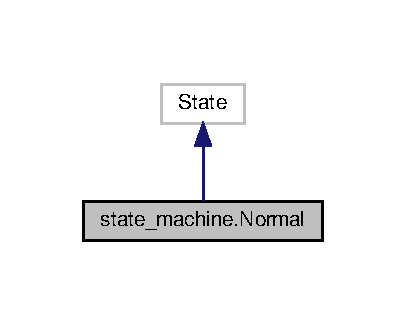
\includegraphics[width=195pt]{classstate__machine_1_1Normal__inherit__graph}
\end{center}
\end{figure}


Collaboration diagram for state\+\_\+machine.\+Normal\+:
\nopagebreak
\begin{figure}[H]
\begin{center}
\leavevmode
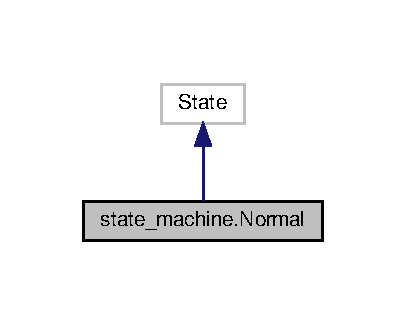
\includegraphics[width=195pt]{classstate__machine_1_1Normal__coll__graph}
\end{center}
\end{figure}
\subsection*{Public Member Functions}
\begin{DoxyCompactItemize}
\item 
\mbox{\Hypertarget{classstate__machine_1_1Normal_acdbc35a37d0350d7805a628048bc3bed}\label{classstate__machine_1_1Normal_acdbc35a37d0350d7805a628048bc3bed}} 
def \hyperlink{classstate__machine_1_1Normal_acdbc35a37d0350d7805a628048bc3bed}{\+\_\+\+\_\+init\+\_\+\+\_\+} (self)
\begin{DoxyCompactList}\small\item\em inizialization \end{DoxyCompactList}\item 
\mbox{\Hypertarget{classstate__machine_1_1Normal_a2930df5f4890ec4b47b2a8e18f9bff08}\label{classstate__machine_1_1Normal_a2930df5f4890ec4b47b2a8e18f9bff08}} 
def \hyperlink{classstate__machine_1_1Normal_a2930df5f4890ec4b47b2a8e18f9bff08}{execute} (self, userdata)
\begin{DoxyCompactList}\small\item\em execution \end{DoxyCompactList}\end{DoxyCompactItemize}
\subsection*{Public Attributes}
\begin{DoxyCompactItemize}
\item 
\hyperlink{classstate__machine_1_1Normal_addf28bcb55a3e1f6bdb118850e164c03}{Random\+Pose}
\begin{DoxyCompactList}\small\item\em 2 outcomes defined \end{DoxyCompactList}\end{DoxyCompactItemize}


\subsection{Detailed Description}
\hyperlink{classstate__machine_1_1Normal}{Normal} state definition. 

Definition at line 53 of file state\+\_\+machine.\+py.



\subsection{Member Data Documentation}
\mbox{\Hypertarget{classstate__machine_1_1Normal_addf28bcb55a3e1f6bdb118850e164c03}\label{classstate__machine_1_1Normal_addf28bcb55a3e1f6bdb118850e164c03}} 
\index{state\+\_\+machine\+::\+Normal@{state\+\_\+machine\+::\+Normal}!Random\+Pose@{Random\+Pose}}
\index{Random\+Pose@{Random\+Pose}!state\+\_\+machine\+::\+Normal@{state\+\_\+machine\+::\+Normal}}
\subsubsection{\texorpdfstring{Random\+Pose}{RandomPose}}
{\footnotesize\ttfamily state\+\_\+machine.\+Normal.\+Random\+Pose}



2 outcomes defined 

set parameter service state = 1

Main Loop subscribe to the command topic generate random target position 

Definition at line 59 of file state\+\_\+machine.\+py.



The documentation for this class was generated from the following file\+:\begin{DoxyCompactItemize}
\item 
src/\hyperlink{state__machine_8py}{state\+\_\+machine.\+py}\end{DoxyCompactItemize}

\hypertarget{classstate__machine_1_1Play}{}\section{state\+\_\+machine.\+Play Class Reference}
\label{classstate__machine_1_1Play}\index{state\+\_\+machine.\+Play@{state\+\_\+machine.\+Play}}


\hyperlink{classstate__machine_1_1Play}{Play} state definition.  




Inheritance diagram for state\+\_\+machine.\+Play\+:
\nopagebreak
\begin{figure}[H]
\begin{center}
\leavevmode
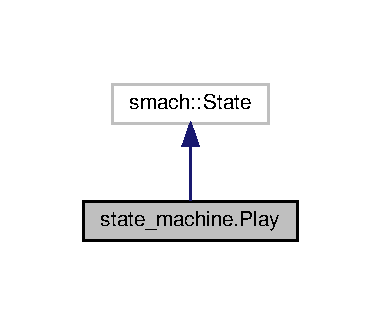
\includegraphics[width=183pt]{classstate__machine_1_1Play__inherit__graph}
\end{center}
\end{figure}


Collaboration diagram for state\+\_\+machine.\+Play\+:
\nopagebreak
\begin{figure}[H]
\begin{center}
\leavevmode
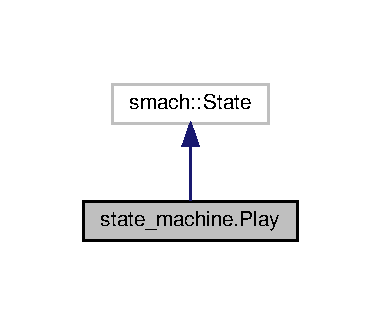
\includegraphics[width=183pt]{classstate__machine_1_1Play__coll__graph}
\end{center}
\end{figure}
\subsection*{Public Member Functions}
\begin{DoxyCompactItemize}
\item 
\mbox{\Hypertarget{classstate__machine_1_1Play_a5993a23d8be7f7b2647f71ede0334957}\label{classstate__machine_1_1Play_a5993a23d8be7f7b2647f71ede0334957}} 
def \hyperlink{classstate__machine_1_1Play_a5993a23d8be7f7b2647f71ede0334957}{\+\_\+\+\_\+init\+\_\+\+\_\+} (self)
\begin{DoxyCompactList}\small\item\em initialization \end{DoxyCompactList}\item 
\mbox{\Hypertarget{classstate__machine_1_1Play_a04168d6842960585b4bbcf58f950547b}\label{classstate__machine_1_1Play_a04168d6842960585b4bbcf58f950547b}} 
def \hyperlink{classstate__machine_1_1Play_a04168d6842960585b4bbcf58f950547b}{execute} (self, userdata)
\begin{DoxyCompactList}\small\item\em Execution. \end{DoxyCompactList}\end{DoxyCompactItemize}
\subsection*{Public Attributes}
\begin{DoxyCompactItemize}
\item 
\mbox{\Hypertarget{classstate__machine_1_1Play_a5817d2ff53ebb02ecf5ceea52ef97a94}\label{classstate__machine_1_1Play_a5817d2ff53ebb02ecf5ceea52ef97a94}} 
\hyperlink{classstate__machine_1_1Play_a5817d2ff53ebb02ecf5ceea52ef97a94}{location}
\begin{DoxyCompactList}\small\item\em 1 outcome defined \+: \hyperlink{classstate__machine_1_1Normal}{Normal} \end{DoxyCompactList}\item 
\mbox{\Hypertarget{classstate__machine_1_1Play_ad666be4461758154b1f51ddc979bca9b}\label{classstate__machine_1_1Play_ad666be4461758154b1f51ddc979bca9b}} 
{\bfseries Pointing\+Gesture}
\end{DoxyCompactItemize}


\subsection{Detailed Description}
\hyperlink{classstate__machine_1_1Play}{Play} state definition. 

Definition at line 121 of file state\+\_\+machine.\+py.



The documentation for this class was generated from the following file\+:\begin{DoxyCompactItemize}
\item 
src/\hyperlink{state__machine_8py}{state\+\_\+machine.\+py}\end{DoxyCompactItemize}

\hypertarget{classstate__machine_1_1Sleep}{}\section{state\+\_\+machine.\+Sleep Class Reference}
\label{classstate__machine_1_1Sleep}\index{state\+\_\+machine.\+Sleep@{state\+\_\+machine.\+Sleep}}


\hyperlink{classstate__machine_1_1Sleep}{Sleep} State definition.  




Inheritance diagram for state\+\_\+machine.\+Sleep\+:
\nopagebreak
\begin{figure}[H]
\begin{center}
\leavevmode
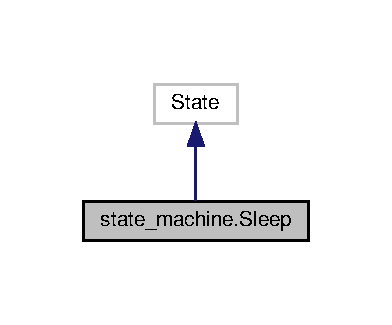
\includegraphics[width=188pt]{classstate__machine_1_1Sleep__inherit__graph}
\end{center}
\end{figure}


Collaboration diagram for state\+\_\+machine.\+Sleep\+:
\nopagebreak
\begin{figure}[H]
\begin{center}
\leavevmode
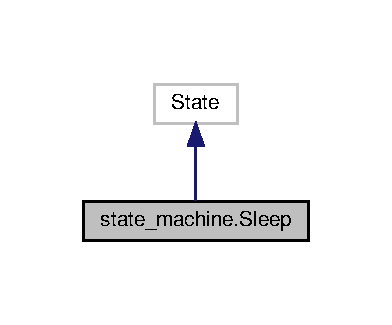
\includegraphics[width=188pt]{classstate__machine_1_1Sleep__coll__graph}
\end{center}
\end{figure}
\subsection*{Public Member Functions}
\begin{DoxyCompactItemize}
\item 
\mbox{\Hypertarget{classstate__machine_1_1Sleep_a473b93a1ddf11f9e664d1fb694ce1a3c}\label{classstate__machine_1_1Sleep_a473b93a1ddf11f9e664d1fb694ce1a3c}} 
def \hyperlink{classstate__machine_1_1Sleep_a473b93a1ddf11f9e664d1fb694ce1a3c}{\+\_\+\+\_\+init\+\_\+\+\_\+} (self)
\begin{DoxyCompactList}\small\item\em Initialization. \end{DoxyCompactList}\item 
\mbox{\Hypertarget{classstate__machine_1_1Sleep_a89527836f1edcefb6467fa9c041fbbfe}\label{classstate__machine_1_1Sleep_a89527836f1edcefb6467fa9c041fbbfe}} 
def \hyperlink{classstate__machine_1_1Sleep_a89527836f1edcefb6467fa9c041fbbfe}{execute} (self, userdata)
\begin{DoxyCompactList}\small\item\em Execution. \end{DoxyCompactList}\end{DoxyCompactItemize}
\subsection*{Public Attributes}
\begin{DoxyCompactItemize}
\item 
\mbox{\Hypertarget{classstate__machine_1_1Sleep_a6bd959627ed45867516c94e3eafc05bb}\label{classstate__machine_1_1Sleep_a6bd959627ed45867516c94e3eafc05bb}} 
\hyperlink{classstate__machine_1_1Sleep_a6bd959627ed45867516c94e3eafc05bb}{home}
\begin{DoxyCompactList}\small\item\em 1 outcome defined \+: \hyperlink{classstate__machine_1_1Normal}{Normal} \end{DoxyCompactList}\end{DoxyCompactItemize}


\subsection{Detailed Description}
\hyperlink{classstate__machine_1_1Sleep}{Sleep} State definition. 

Definition at line 94 of file state\+\_\+machine.\+py.



The documentation for this class was generated from the following file\+:\begin{DoxyCompactItemize}
\item 
src/\hyperlink{state__machine_8py}{state\+\_\+machine.\+py}\end{DoxyCompactItemize}

\chapter{File Documentation}
\hypertarget{Commander_8py}{}\section{src/\+Commander.py File Reference}
\label{Commander_8py}\index{src/\+Commander.\+py@{src/\+Commander.\+py}}


This node generates and sends the command.  


\subsection*{Functions}
\begin{DoxyCompactItemize}
\item 
\mbox{\Hypertarget{Commander_8py_a21fd1006eebcfe7a9ff3ab55d94a6715}\label{Commander_8py_a21fd1006eebcfe7a9ff3ab55d94a6715}} 
def \hyperlink{Commander_8py_a21fd1006eebcfe7a9ff3ab55d94a6715}{Commander.\+User\+Action} ()
\begin{DoxyCompactList}\small\item\em User\+Action Function. \end{DoxyCompactList}\end{DoxyCompactItemize}


\subsection{Detailed Description}
This node generates and sends the command. 

Details\+: The command is randomply choosen between play and sleep. If play is selected then it generates randomly the target positions as well. 
\hypertarget{Display_8py}{}\section{src/\+Display.py File Reference}
\label{Display_8py}\index{src/\+Display.\+py@{src/\+Display.\+py}}


This node displays the target Position.  


\subsection*{Functions}
\begin{DoxyCompactItemize}
\item 
\mbox{\Hypertarget{Display_8py_a09e8af8fdd997f1a3accfeadf77d98b6}\label{Display_8py_a09e8af8fdd997f1a3accfeadf77d98b6}} 
def \hyperlink{Display_8py_a09e8af8fdd997f1a3accfeadf77d98b6}{Display.\+odom\+Callback} (data)
\begin{DoxyCompactList}\small\item\em odom\+Callback \+: callback for new Target Position \end{DoxyCompactList}\item 
\mbox{\Hypertarget{Display_8py_aaac75616364a30e299644a824211ddc3}\label{Display_8py_aaac75616364a30e299644a824211ddc3}} 
def \hyperlink{Display_8py_aaac75616364a30e299644a824211ddc3}{Display.\+Read\+Position} ()
\begin{DoxyCompactList}\small\item\em Read\+Position function. \end{DoxyCompactList}\end{DoxyCompactItemize}
\subsection*{Variables}
\begin{DoxyCompactItemize}
\item 
\mbox{\Hypertarget{Display_8py_a08ac302295d8e97a0e72546b508747be}\label{Display_8py_a08ac302295d8e97a0e72546b508747be}} 
{\bfseries Display.\+New\+Target} = Point()
\item 
\mbox{\Hypertarget{Display_8py_a171c1d9b9a41d2602dd604af8733b34b}\label{Display_8py_a171c1d9b9a41d2602dd604af8733b34b}} 
\hyperlink{Display_8py_a171c1d9b9a41d2602dd604af8733b34b}{Display.\+old\+\_\+\+Position} = Point()
\begin{DoxyCompactList}\small\item\em initialization Position \end{DoxyCompactList}\item 
\mbox{\Hypertarget{Display_8py_ae8848feed57b8de85f2936b3b2b5d80e}\label{Display_8py_ae8848feed57b8de85f2936b3b2b5d80e}} 
{\bfseries Display.\+x}
\item 
\mbox{\Hypertarget{Display_8py_a219a78a85aa3669683f5fc7cc53131ad}\label{Display_8py_a219a78a85aa3669683f5fc7cc53131ad}} 
{\bfseries Display.\+y}
\item 
\mbox{\Hypertarget{Display_8py_a3d42727f8bd08916f337a313428fbf42}\label{Display_8py_a3d42727f8bd08916f337a313428fbf42}} 
{\bfseries Display.\+z}
\end{DoxyCompactItemize}


\subsection{Detailed Description}
This node displays the target Position. 

Details\+: It subsscribe to a newtargetposition topic and publishes what the robot is doing 
\hypertarget{state__machine_8py}{}\section{src/state\+\_\+machine.py File Reference}
\label{state__machine_8py}\index{src/state\+\_\+machine.\+py@{src/state\+\_\+machine.\+py}}


This node implements a state machine.  


\subsection*{Classes}
\begin{DoxyCompactItemize}
\item 
class \hyperlink{classstate__machine_1_1Normal}{state\+\_\+machine.\+Normal}
\begin{DoxyCompactList}\small\item\em \hyperlink{classstate__machine_1_1Normal}{Normal} state definition. \end{DoxyCompactList}\item 
class \hyperlink{classstate__machine_1_1Sleep}{state\+\_\+machine.\+Sleep}
\begin{DoxyCompactList}\small\item\em \hyperlink{classstate__machine_1_1Sleep}{Sleep} State definition. \end{DoxyCompactList}\item 
class \hyperlink{classstate__machine_1_1Play}{state\+\_\+machine.\+Play}
\begin{DoxyCompactList}\small\item\em \hyperlink{classstate__machine_1_1Play}{Play} state definition. \end{DoxyCompactList}\end{DoxyCompactItemize}
\subsection*{Functions}
\begin{DoxyCompactItemize}
\item 
\mbox{\Hypertarget{state__machine_8py_a366eb29323af9f65f6d2aa4907cc5c4d}\label{state__machine_8py_a366eb29323af9f65f6d2aa4907cc5c4d}} 
def \hyperlink{state__machine_8py_a366eb29323af9f65f6d2aa4907cc5c4d}{state\+\_\+machine.\+Generate\+Random\+Position} ()
\begin{DoxyCompactList}\small\item\em Generate\+Random\+Position function. \end{DoxyCompactList}\item 
\mbox{\Hypertarget{state__machine_8py_a4943590f488a3f9c5cfff37b4a665e7d}\label{state__machine_8py_a4943590f488a3f9c5cfff37b4a665e7d}} 
def \hyperlink{state__machine_8py_a4943590f488a3f9c5cfff37b4a665e7d}{state\+\_\+machine.\+commcallback} (data)
\begin{DoxyCompactList}\small\item\em commcallback \+: callback for the command \end{DoxyCompactList}\item 
\mbox{\Hypertarget{state__machine_8py_a79d0a5f93940f58b317266b50576e96a}\label{state__machine_8py_a79d0a5f93940f58b317266b50576e96a}} 
def \hyperlink{state__machine_8py_a79d0a5f93940f58b317266b50576e96a}{state\+\_\+machine.\+Person\+Positioncallback} (pose)
\begin{DoxyCompactList}\small\item\em Person\+Positioncallback \+: callback for the Person Position. \end{DoxyCompactList}\item 
\mbox{\Hypertarget{state__machine_8py_a5cef0355936441fecaeb0cdce52b0c1f}\label{state__machine_8py_a5cef0355936441fecaeb0cdce52b0c1f}} 
def \hyperlink{state__machine_8py_a5cef0355936441fecaeb0cdce52b0c1f}{state\+\_\+machine.\+Pointing\+Gesturecallback} (pose2)
\begin{DoxyCompactList}\small\item\em Pointing\+Gesturecallback\+: callback for the Pointed Location. \end{DoxyCompactList}\item 
\mbox{\Hypertarget{state__machine_8py_a5c680ce705e6052fa07c6cece21743d0}\label{state__machine_8py_a5c680ce705e6052fa07c6cece21743d0}} 
def \hyperlink{state__machine_8py_a5c680ce705e6052fa07c6cece21743d0}{state\+\_\+machine.\+main} ()
\begin{DoxyCompactList}\small\item\em Main Function definition. \end{DoxyCompactList}\end{DoxyCompactItemize}
\subsection*{Variables}
\begin{DoxyCompactItemize}
\item 
\mbox{\Hypertarget{state__machine_8py_ab732f678633e5517fa0bdc3f5acb5e81}\label{state__machine_8py_ab732f678633e5517fa0bdc3f5acb5e81}} 
{\bfseries state\+\_\+machine.\+pose} = Point()
\item 
\mbox{\Hypertarget{state__machine_8py_a3d998d702fb3cd993d11016395ed2edd}\label{state__machine_8py_a3d998d702fb3cd993d11016395ed2edd}} 
{\bfseries state\+\_\+machine.\+userdata} = String()
\item 
\mbox{\Hypertarget{state__machine_8py_aa1bd9d2e1822f6552d375afa39a4f214}\label{state__machine_8py_aa1bd9d2e1822f6552d375afa39a4f214}} 
{\bfseries state\+\_\+machine.\+Person\+Position} = Point()
\item 
\mbox{\Hypertarget{state__machine_8py_a5c28d192bed58b1dd815737bf108bb83}\label{state__machine_8py_a5c28d192bed58b1dd815737bf108bb83}} 
{\bfseries state\+\_\+machine.\+Pointing\+Gesture} = Point()
\end{DoxyCompactItemize}


\subsection{Detailed Description}
This node implements a state machine. 

Details\+: It is the main node\+: it receives commands from the commander node, implements the state machine and sends the target positions to display node. 
%--- End generated contents ---

% Index
\backmatter
\newpage
\phantomsection
\clearemptydoublepage
\addcontentsline{toc}{chapter}{Index}
\printindex

\end{document}
